\documentclass{article}
\usepackage{amssymb}
\usepackage{tikz}
\usetikzlibrary{arrows,automata}
\newcounter{problem}
\newcounter{solution}

\newcommand\Problem{%
  \stepcounter{problem}%
  \textbf{\theproblem.}~%
  \setcounter{solution}{0}%
}

\newcommand\TheSolution{%
  \textbf{Solution \theproblem:}\\%
}

\newcommand\ASolution{%
  \stepcounter{solution}%
  \textbf{Solution \theproblem.\thesolution:}\\%
}
\parindent 0in
\parskip 1em
\begin{document}

\begin{center}
\fbox{\fbox{\parbox{4in}{\centering Assignment 3 by Lucas Karlsson}}}
\end{center}

\Problem Construct an NFA (without $\epsilon$-transitions) that recognises the same language 
over $\{0,1\}$ as the rgular expression $(0+01^*)^*(\epsilon+1)1(\epsilon+0+1)^*.$ 

\TheSolution To construct this NFA I'd first like to rewrite or simplify the regular expression, there
is no easy way of doing this have I come to find the hard way. But I'm going to give it a shot!

$(0+01^*)^* = (01^*)^*$ Because it has to start with either nothing or a zero followed by zero or more ones
and doing all of this zero or more times.

We now have $(01^*)^*(\epsilon+1)1(\epsilon+0+1)^*$ and $(\epsilon+1)1 = (1+11)$ because of distributative 
laws, basically we either have one 1 or two 1's.

We can also simplify $(\epsilon+0+1)^*$ which is the same thing as $(0+1)^*$ because $0\epsilon1$ is the same 
thing as $01$

Our regular expression will now be $(01^*)^*(1+11)(0+1)^*$ we can immediatelly see that $(1+11)$ is can be 
simplified further because our $11$ case is already covered by the $(0+1)^*$ so we can simply rewrite the 
expression again to $(01^*)^*1(0+1)^*$. In words we can explain this as the paragraph below and we can easily 
create a simple NFA as seen below.
\begin{center}
  "Starts with either zero or more 0's followed by atleast one 1 then any of 0 or 1 zero or more times"
\end{center}

\begin{center}
 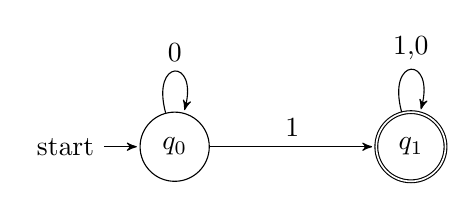
\begin{tikzpicture}[>=stealth',shorten >=1pt,auto,node distance=3cm]
   \node[initial,state]   (q0)                     {$q_0$};
   \node[accepting,state]           (q1) [right of=q0]       {$q_1$};

   \path[->] (q0) edge                node {1} (q1)
                  edge [loop above]   node {0} (q0)
             (q1) edge [loop above]   node {1,0} (q1);

 \end{tikzpicture}
\end{center}

This NFA satisfies the regular expression in question and recongnises the same language over $\{0,1\}$
You can also find this NFA in the file \textbf{ass3point1.jff}.

\newpage

\Problem Construct a regular expression for the language over $\{0,1\}$ that consists of 
every string $w \in \{0,1\}^*$ that satisfies conditions in the question.

\TheSolution We need to satisfy the properities $|w| \geqslant 2$, the first and last symbol 
in w must be 1 and the string 00 must not occur in w.

What I did is first create a NFA satisfying the properties, which looks as below:


\begin{center}
 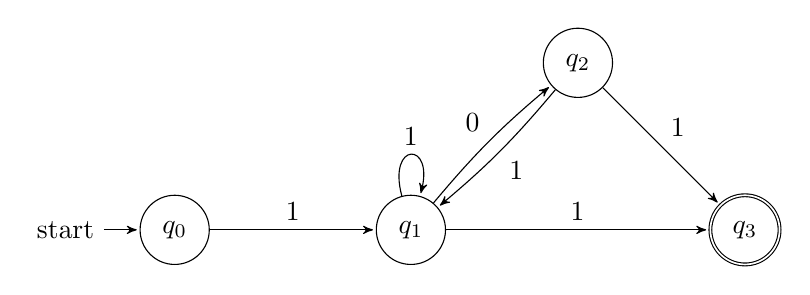
\begin{tikzpicture}[>=stealth',shorten >=1pt,auto,node distance=3cm]
   \node[initial,state]   (q0)                     {$q_0$};
   \node[state]           (q1) [right of=q0]       {$q_1$};
   \node[state]           (q2) [above right of=q1] {$q_2$};
   \node[state,accepting] (q3) [below right of=q2] {$q_3$};

   \path[->] (q0) edge                node {1} (q1)
             (q1) edge [loop above]   node {1} (q1)
                  edge [bend left =5] node {0} (q2)
                  edge                node {1} (q3)
             (q2) edge [bend left =5] node {1} (q1)
                  edge                node {1} (q3);

 \end{tikzpicture}
\end{center}

Now we can start converting this NFA to a regular expression this can be done using a method 
that eliminates states replacing them with regular expressions.

Step 1, we can now prepare to remove states. This is easy because we have no 
states coming in to our initial states and no states coming out of our final state, that 
basically translates into we don't need to do something before we start removing states.
We start by removing the $q_2$ state. Our automata will look like this:

\begin{center}
 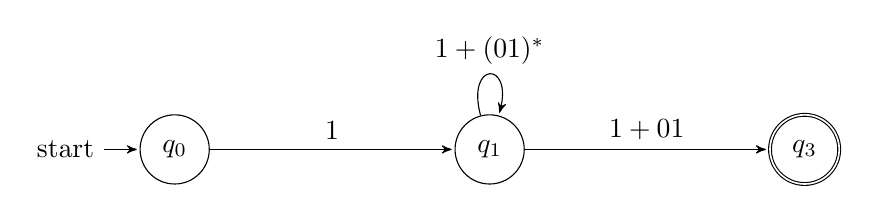
\begin{tikzpicture}[>=stealth',shorten >=1pt,auto,node distance=4cm]
   \node[initial, state]  (q0)                     {$q_0$};
   \node[state]           (q1) [right of=q0]       {$q_1$};
   \node[state,accepting] (q3) [right of=q1] {$q_3$};

   \path[->] (q0) edge                node {1} (q1)
             (q1) edge [loop above]   node {$1 + (01)^*$} (q1)
                  edge                node {$1 + 01$} (q3);
 \end{tikzpicture}
\end{center}

The only thing we now have left to remove is the $q_1$ state, this would look as following:

\begin{center}
 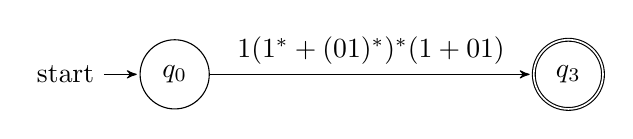
\begin{tikzpicture}[>=stealth',shorten >=1pt,auto,node distance=5cm]
   \node[initial, state]  (q0)                     {$q_0$};
   \node[state,accepting] (q3) [right of=q0] {$q_3$};

   \path[->] (q0) edge node {$1(1^*+(01)^*)^*(1+01)$} (q3);
 \end{tikzpicture}
\end{center}

We are done here but we can simplify the regular expression further because $(1^*+(01)^*)^* = (1+01)^*$
and our final regular expression will then be: 
\[1(1+01)^*(1+01)\]
\newpage

\Problem Convert the $\epsilon$-NFA in the question to an equivalent DFA.

\begin{table}[h!]
  \centering
  \begin{tabular}{c c c c c}
    &\textbf{$State$}& $\epsilon$ &\textbf{a}&\textbf{b}\\
    $\to$        & $s_0$ & $\emptyset$ & $\{s_1\}$ & $\{s_0,s_2\}$\\
    \hfill       & $s_1$ & $\{s_2\}$ & $\{s_4\}$ & $\{s_3\}$\\
    \hfill       & $s_2$ & $\emptyset$ & $\{s_1,s_4\}$ & $\{s_3\}$\\
    \hfill       & $s_3$ & $\{s_5\}$ & $\{s_4,s_5\}$ & $\emptyset$\\
    \hfill       & $s_4$ & $\{s_3\}$ & $\emptyset$ & $\{s_5\}$\\
    \hfill     * & $s_5$ & $\emptyset$ & $\{s_5\}$ & $\{s_5\}$\\
  \end{tabular}
\end{table}

\TheSolution I'm going to start by converting the $\epsilon$-NFA to a equivalent NFA this can be
done by everytime we find a $\epsilon$ for every occurence of the state we add the states in the $\epsilon$
transition. You can also express this with $\delta (q_0, a) = \delta_{hat} (q_0, a)$. Our new table will look 
this:

\begin{table}[h!]
  \centering
  \begin{tabular}{c c c c}
    &\textbf{$State$}&\textbf{a}&\textbf{b} \\
    $\to$    & $s_0$ & $s_1,s_2$ & $s_0,s_2$ \\
             & $s_1$ & $s_3,s_4,s_5$ & $s_3,s_5$ \\
             & $s_2$ & $s_1,s_2,s_3,s_4,s_5$ & $s_3,s_5$ \\
             & $s_3$ & $s_3,s_4,s_5$ & $\emptyset$ \\
             & $s_4$ & $\emptyset$ & $s_5$ \\
    \hfill * & $s_5$ & $s_5$ & $s_5$ \\ [0.5ex]
  \end{tabular}
\end{table}

Now we can create a DFA using this NFA by starting at $s_0$ and doing $\delta (s_0,a)$ and $\delta (s_0,b)$
and using the states that we get from the calculation doing the same $\delta$ function for a and b for them. 
I will do the calculations here in latex and filling in my table as I go along.

$\delta(s_0,a) = \delta_n (s_0,a) = \{s_1,s_2\}$ \newline
$\delta(s_0,b) = \delta_n (s_0,b) = \{s_0,s_2\}$ 

$\delta(s_1s_2,a) = \delta_n (s_1,a) \cup \delta_n (s_2,a) = \{s_1,s_2,s_3,s_4,s_5\}$\newline
$\delta(s_1s_2,b) = \delta_n (s_1,b) \cup \delta_n (s_2,b) = \{s_3,s_5\}$\newline
$\delta(s_0s_2,a) = \delta_n (s_0,a) \cup \delta_n (s_2,a) = \{s_1,s_2,s_3,s_4,s_5\}$ \newline
$\delta(s_0s_2,b) = \delta_n (s_0,b) \cup \delta_n (s_2,b) = \{s_0,s_2,s_3,s_5\}$

$\delta(s_1s_2s_3s_4s_5,a) = \delta_n (s_1,a) \cup \delta_n (s_2,a) \cup \delta_n (s_3,a) \cup \delta_n (s_4,a) \cup \delta_n (s_5,a) = \{s_1,s_2,s_3,s_4,s_5\}$ \newline
$\delta(s_1s_2s_3s_4s_5,b) = \delta_n (s_1,b) \cup \delta_n (s_2,b) \cup \delta_n (s_3,b) \cup \delta_n (s_4,b) \cup \delta_n (s_5,b) = \{s_3,s_5\}$\newline
$\delta(s_3s_5,a) = \delta_n (s_3,a) \cup \delta_n (s_5,a) = \{s_3,s_4,s_5\}$\newline
$\delta(s_3s_5,b) = \delta_n (s_3,b) \cup \delta_n (s_5,b) = \{s_5\}$\newline
$\delta(s_0s_2s_3s_5,a) = \delta_n (s_0,a) \cup \delta_n (s_2,a) \cup \delta_n (s_3,a) \cup \delta_n (s_5,a) = 
\{s_1,s_2,s_3,s_4,s_5\}$\newline
$\delta(s_0s_2s_3s_5,b) = \delta_n (s_0,b) \cup \delta_n (s_2,b) \cup \delta_n (s_3,b) \cup \delta_n (s_5,b) = 
\{s_0,s_2,s_3,s_5\}$

$\delta(s_3s_4s_5,a) = \delta_n (s_3,a) \cup \delta_n (s_4,a) \cup \delta_n (s_5,a) = \{s_3,s_4,s_5\}$ \newline
$\delta(s_3s_4s_5,b) = \delta_n (s_3,b) \cup \delta_n (s_4,b) \cup \delta_n (s_5,b) = \{s_5\}$\newline
$\delta(s_5,a) = \delta_n (s_5,a) = \{s_5\}$\newline
$\delta(s_5,b) = \delta_n (s_5,b) = \{s_5\}$

\begin{table}[h!]
  \centering
  \begin{tabular}{c c c c}
    &\textbf{$State$}&\textbf{a}&\textbf{b}\\ [0.5ex]
\hfill $\to$ ($q_0$) & $s_0$ & $s_1s_2$ & $s_0s_2$ \\
\hfill       ($q_1$) & $s_1s_2$ & $s_1s_2s_3s_4s_5$ & $s_3s_5$ \\
\hfill       ($q_2$) & $s_0s_2$ & $s_1s_2s_3s_4s_5$ & $s_0s_2s_3s_5$ \\ 
\hfill     * ($q_3$) & $s_1s_2s_3s_4s_5$ & $s_1s_2s_3s_4s_5$ & $s_3s_5$ \\
\hfill     * ($q_4$) & $s_3s_5$ & $s_3s_4s_5$ & $s_5$ \\
\hfill     * ($q_5$) & $s_0s_2s_3s_5$ & $s_1s_2s_3s_4s_5$ & $s_0s_2s_3s_5$ \\
\hfill     * ($q_6$) & $s_3s_4s_5$ & $s_3s_4s_5$ & $s_5$ \\
\hfill     * ($q_7$) & $s_5$ & $s_5$ & $s_5$ \\
  
  \end{tabular}
\end{table}

This will be our final construction, we have now created a DFA from the given $\epsilon$-NFA. This DFA can also be found in the file \textbf{ass3point3.jff}.

\newpage
\Problem Convert the NFA to an equivalent regular expression
\begin{center}
 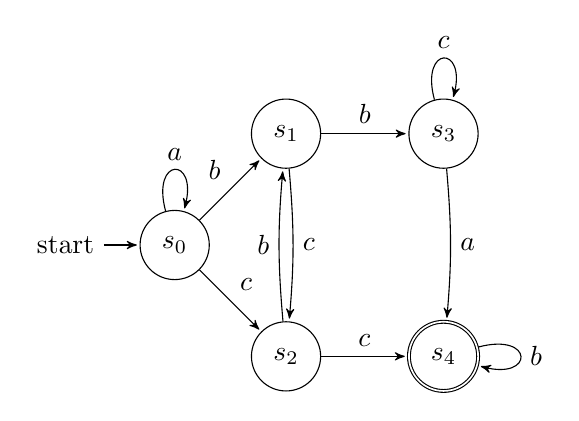
\begin{tikzpicture}[>=stealth',shorten >=1pt,auto,node distance=2cm]
   \node[initial,state]   (s0)                     {$s_0$};
   \node[state]           (s1) [above right of=s0] {$s_1$};
   \node[state]           (s2) [below right of=s0] {$s_2$};
   \node[state]           (s3) [right of=s1]       {$s_3$};
   \node[state,accepting] (s4) [right of=s2]       {$s_4$};

   \path[->] (s0) edge                node {$c$} (s2)
                  edge                node {$b$} (s1)
                  edge [loop above]   node {$a$} (s0)
             (s1) edge                node {$b$} (s3)
                  edge [bend left =5] node {$c$} (s2)
             (s2) edge [bend left =5] node {$b$} (s1)
                  edge                node {$c$} (s4)
             (s3) edge [bend left =5] node {$a$} (s4)
                  edge [loop above]   node {$c$} (s3)
             (s4) edge [loop right]   node {$b$} (s4);
 \end{tikzpicture} 
\end{center} 

\TheSolution To start off converting this NFA I'm going to establish the technique I'm going to use. It is
indeed quite similar to the one I used in \textbf{Solution 2} but we need to do some extra steps.
I can immediatelly see that because I have \textbf{in-going} edges on my initial state which needs to be 
fixed. I also have \textbf{outgoing} edges on my accepting state, this will also need correcection.

\textbf{Step 1} Add incoming $\epsilon$-transistion and new accepting state.
\begin{center}
 \begin{tikzpicture}[>=stealth',shorten >=1pt,auto,node distance=2cm]
   \node[initial,state]   (q0) [left of=s0]        {$q_0$};
   \node[state]           (s0)                     {$s_0$};
   \node[state]           (s1) [above right of=s0] {$s_1$};
   \node[state]           (s2) [below right of=s0] {$s_2$};
   \node[state]           (s3) [right of=s1]       {$s_3$};
   \node[state]           (s4) [right of=s2]       {$s_4$};
   \node[accepting,state] (q1) [right of=s4]       {$q_1$};

   \path[->] (s0) edge                node {$c$} (s2)
                  edge                node {$b$} (s1)
                  edge [loop above]   node {$a$} (s0)
             (s1) edge                node {$b$} (s3)
                  edge [bend left =5] node {$c$} (s2)
             (s2) edge [bend left =5] node {$b$} (s1)
                  edge                node {$c$} (s4)
             (s3) edge                node {$a$} (s4)
                  edge [loop above]   node {$c$} (s3)
             (s4) edge [loop below]   node {$b$} (s4)
                  edge                node {$\epsilon$} (q1)
             (q0) edge                node {$\epsilon$} (s0);
 \end{tikzpicture} 
\end{center} 

\newpage
\textbf{Step 2} We can now start removing states and replacing them with regular expressions. I'd like to 
remove $s_3$ first. This can easily be done by adding the $bc^*a$ edge.

\begin{center}
 \begin{tikzpicture}[>=stealth',shorten >=1pt,auto,node distance=2cm]
   \node[initial,state]   (q0) [left of=s0]        {$q_0$};
   \node[state]           (s0)                     {$s_0$};
   \node[state]           (s1) [above right of=s0] {$s_1$};
   \node[state]           (s2) [below right of=s0] {$s_2$};
   \node[state]           (s4) [right of=s2]       {$s_4$};
   \node[accepting,state] (q1) [right of=s4]       {$q_1$};

   \path[->] (s0) edge                node {$c$} (s2)
                  edge                node {$b$} (s1)
                  edge [loop above]   node {$a$} (s0)
             (s1) edge                node {$bc^*a$} (s4)
                  edge [bend left =5] node {$c$} (s2)
             (s2) edge [bend left =5] node {$b$} (s1)
                  edge                node {$c$} (s4)
             (s4) edge [loop below]   node {$b$} (s4)
                  edge                node {$\epsilon$} (q1)
             (q0) edge                node {$\epsilon$} (s0);
 \end{tikzpicture} 
\end{center} 

\textbf{Step 3} Next I'd like to remove the $s_1$ state, this is a bit harder but can be done by
adding $bc$ loop on $s_2$ and changing the $s_0s_2$ edge to $c + bc$ and adding $s_0s_4$ edge $(cb+b)bc^*a$.

\begin{center}
 \begin{tikzpicture}[>=stealth',shorten >=1pt,auto,node distance=2.5cm]
   \node[initial,state]   (q0) [left of=s0]        {$q_0$};
   \node[state]           (s0)                     {$s_0$};
   \node[state]           (s2) [right of=s0]       {$s_2$};
   \node[state]           (s4) [right of=s2]       {$s_4$};
   \node[accepting,state] (q1) [right of=s4]       {$q_1$};

   \path[->] (s0) edge                node {$c + bc$} (s2)
                  edge [loop above]   node {$a$} (s0)
                  edge [bend left =55]node {$(cb + b)bc^*a$} (s4)
             (s2) edge [loop above]   node {$bc$} (s1)
                  edge                node {$c$} (s4)
             (s4) edge [loop above]   node {$b$} (s4)
                  edge                node {$\epsilon$} (q1)
             (q0) edge                node {$\epsilon$} (s0);
 \end{tikzpicture} 
\end{center} 

\textbf{Step 4} Now we are almost done and can simply remove the $s_2$ state and join our two regular
expression with $(bc)^*$ in the middle.

\begin{center}
 \begin{tikzpicture}[>=stealth',shorten >=1pt,auto,node distance=2.5cm]
   \node[initial,state]   (q0) [left of=s0]        {$q_0$};
   \node[state]           (s0)                     {$s_0$};
   \node[state]           (s4) [right of=s2]       {$s_4$};
   \node[accepting,state] (q1) [right of=s4]       {$q_1$};

   \path[->] (s0) edge [bend left =55]   node {$((cb+b)(cb)^*bc^*a)+((c+bc)(bc)^*c)$} (s4)
                  edge [loop above]   node {$a$} (s0)
             (s4) edge [loop above]   node {$b$} (s4)
                  edge                node {$\epsilon$} (q1)
             (q0) edge                node {$\epsilon$} (s0);
 \end{tikzpicture} 
\end{center} 

\newpage
\textbf{Step 5} Only thing left now is removing $s_0$ and $s_4$, easy peasy lemon squeezy. Our final 
regular expression and our answer to the question will be the one inbetween $q_0$ and $q_1$

\begin{center}
 \begin{tikzpicture}[>=stealth',shorten >=1pt,auto,node distance=2.5cm]
   \node[initial,state]   (q0) [left of=s0]        {$q_0$};
   \node[accepting,state] (q1) [right of=s4]       {$q_1$};
   \path[->] (q0) edge node {$a^*((cb+b)(cb)^*bc^*a)+((c+bc)(bc)^*c)b^*$} (q1);
 \end{tikzpicture} 
\end{center} 

\end{document}
